\documentclass[10pt,a4paper]{article}
\usepackage[utf8]{inputenc}
\usepackage[spanish]{babel}
\usepackage{amsmath}
\usepackage{amsfonts}
\usepackage{amssymb}
\usepackage{makeidx}
\usepackage{graphicx}
\usepackage{lmodern}
\usepackage{kpfonts}
\usepackage{fourier}
\usepackage[hidelinks]{hyperref}
\usepackage[left=2cm,right=2cm,top=2cm,bottom=2cm]{geometry}
\title{Giro de un motor de corriente directa.}
\author{Luis Angel Torres Pinto. }\\
\begin{document}
\maketitle
\centering

\includegraphics[scale=2.10]{upzmg.jpg}\\
\raggedright
\newpage
\section{Principio de funcionamiento.}
El principio de funcionamiento de los motores eléctricos de corriente directa se basa en la repulsión que ejercen los polos magnéticos de un electroimán que se encuentra montado en un eje. Este electroimán se denomina "rotor" y su eje le permite girar libremente entre los polos electroimán norte y sur del imán permanente situado dentro de la carcasa o cuerpo del motor.\\
Cuando la corriente eléctrica circula por la bobina de este electroimán giratorio, el campo electromagnético que se genera interactúa con el campo magnético del imán permanente. Si los polos del imán permanente y del electroimán giratorio coinciden, se produce un rechazo y un torque magnético o par de fuerza que provoca que el rotor rompa la inercia y comience a girar sobre su eje en el mismo sentido de las manecillas del reloj en unos casos, o en sentido contrario, de acuerdo con la forma que se encuentre conectada al circuito la pila o la batería.
\section{Función del colector o conmutador en el motor de C.D.}
En el motor de corriente directa el colector o conmutador sirve para conmutar o cambiar constantemente, el sentido de circulación de la corriente eléctrica a través del enrollado de la bobina del rotor  cada  vez, que completa media vuelta. De esa forma el polo norte del electroimán coincidirá siempre con el también. polo norte del imán permanente y el polo sur con el polo sur del propio imán. Al coincidir siempre dos polos magnéticos, que en todo momento van a ser iguales, se produce un rechazo constante entre ambos, lo que permite al rotor mantenerse girando ininterrumpidamente sobre su eje durante todo el tiempo que se encuentre conectado a la corriente eléctrica.\\
\centering
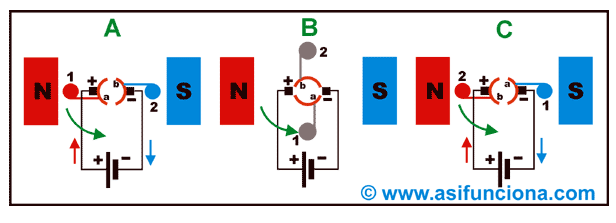
\includegraphics[scale=.60]{motor.png}\\
\raggedright
Tal como vemos, en “A” de la figura, la bobina del electroimán se encuentra colocada entre los polos norte “N” y sur “S” del campo magnético del imán permanente. A su vez, el polo positivo (+) de la batería se encuentra conectado siguiendo el sentido convencional de la corriente (del signo positivo al negativo) en la mitad “a” del colector a través de la escobilla identificada también con el signo (+). De esa forma la mitad de la bobina de color rojo (1) se energiza positivamente para formar el polo norte “N”, mientras que la otra mitad, la de color azul (2) se energiza negativamente para formar el polo sur “S”.\\

Como resultado, cuando en el electroimán se forma el polo norte, de inmediato el también polo norte del imán permanente lo rechaza. Al mismo tiempo el polo sur que se forma en el extremo opuesto, es rechazado igualmente por el polo sur del propio imán; por tanto se produce una fuerza de repulsión en ambos extremos del rotor al enfrentarse y coincidir con dos polos iguales en el imán permanente. Si bajo esas condiciones aplicamos la “Regla de la mano izquierda” y tomamos como referencia, por ejemplo, la parte de la bobina donde se ha formado el polo norte en el electroimán, comprobaremos que al romper la inercia inicial, comenzará a girar en dirección contraria a las manecillas del reloj, como indica la flecha de color verde.\\

Una vez que la bobina del electroimán gira y asume una posición vertical (como se muestra en la parte “B” de la ilustración), las escobillas dejan de hacer contacto con ambos segmentos del colector. En esa posición neutra la corriente que suministra la batería deja de circular y la bobina se desenergiza, por lo que ambos extremos del electroimán pierden momentáneamente sus polos magnéticos. No obstante, debido a la fuerza de inercia o impulso de giro que mantiene el electroimán, esa posición la rebasa de inmediato y sus extremos pasan a ocupar la posición opuesta a la que tenían, tal como se muestra en la parte “C” de la misma ilustración.\\

Ahora en “C” se puede ver que la mitad de la bobina que anteriormente tenía color azul (2) con polaridad sur cuando se encontraba situada a la derecha del eje del rotor pasa a ocupar la parte izquierda junto con la mitad (b) del colector al que se encuentra conectada. Esa parte de la bobina que ha girado, al ocupar ahora la posición opuesta, se convierte en el polo norte (2) del electroimán por lo que es rechazado de nuevo por el polo norte del imán permanente, que como ya se explicó se encuentra fijo al cuerpo del motor. Seguidamente el electroimán, al continuar girando y dar otra media vuelta, pasa de nuevo por la zona neutra (como en “B”) repitiéndose de nuevo el mismo ciclo. Esos cambios continuos en los polos del electroimán del rotor que proporciona el colector, son los que permiten que se mantenga girando de forma ininterrumpida mientras se mantenga energizado.\\
\centering
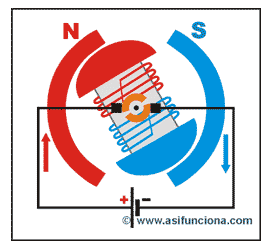
\includegraphics[scale=.80]{gi.png}\\
\raggedright
En esta figura se muestra el funcionamiento de un motor común bipolar de corriente directa. Como se puede observar, éste consta de un imán permanente en forma de semicírculo, dividido en dos partes fijas al cuerpo del motor. La parte de color rojo del imán corresponde al polo norte “N” y la azul al polo sur “S”. También encontramos un electroimán que a modo de rotor gira entre los polos magnéticos del imán permanente. En el eje del rotor se muestra un colector dividido en dos segmentos y dos escobillas haciendo contacto con los mismos. La batería se encuentra conectada de tal forma que la corriente eléctrica fluye en el sentido convencional con el polo positivo (+) conectado a la escobilla derecha y el polo negativo (–) a la escobilla izquierda. Cada escobilla hace pleno contacto con las secciones del colector, incluso mientras el rotor se encuentra girando.\\

Como la bobina del rotor se encuentra conectada a ambos segmentos del colector, éste se energiza con la corriente eléctrica directa que suministra la fuente de fuerza electromotriz (F.E.M.) (en este caso la batería), que le llega a través de las escobillas. De esa forma la corriente la recibe el colector a través de la escobilla izquierda identificada con el signo (+), recorre las espiras correspondientes a esa mitad de la bobina del electroimán (de color rojo) y continúa recorriendo las espiras de la mitad derecha (de color azul) para retornar, finalmente, a la batería por su polo negativo (–), completando así el circuito eléctrico del motor.\\

Cuando la corriente eléctrica comienza a fluir por la parte correspondiente a las espiras de color rojo, el electroimán adquiere polaridad norte “N” en ese extremo y polaridad sur “S” en el extremo opuesto representado por las espiras de color azul.\\
\section{Referencias }
\url{http://www.asifunciona.com/electrotecnia/af_motor_cd/af_motor_cd_7.htm}
\end{document}